\documentclass[../Analysis-3.tex]{subfiles}

\tolerance=1
\emergencystretch=\maxdimen
\hyphenpenalty=10000
\hbadness=10000

\begin{document}
\chapter*{Lecture 6} %Set chapter name
\addcontentsline{toc}{chapter}{Lecture 6} %Set chapter title
\setcounter{chapter}{6} %Set chapter counter
\setcounter{section}{0}
\setcounter{equation}{0}
\setcounter{figure}{0}


\section{Partial Derivatives}

Now, we discuss the notion of partial derivatives. This tries to treat differentiation of functions with multiple arguments in the 1-variable setting. This construction ends up being an indispensable tool in the computation of the Total derivative in the standard basis.\\[0.2 cm]

Consider a function $f:\Op{n} \rightarrow\R$ and a point $a \in \Op{n}$, and fix $1 \leq i \leq n$. Now, we define functions $\eta_i : (-\varepsilon, \varepsilon) \rightarrow \R$ such that $\eta(t) = f(a + te_i)$ for all $t \in (-\varepsilon, \varepsilon)$.

\begin{Def}{Partial Derivatives}{}
  For the given function $f:\Op{n} \rightarrow\R$, the partial derivatives of $f$ with respect to the co-ordinate $x_i$ is given by:
  \[
    f_{x_i}(a) \equiv \pdv{f}{x_i}\/(a) \mathrel{\mathop:}=  \frac{d\eta_i}{dt}(a) = \lim_{t \to 0} \frac{f(a+te_i) - f(a)}{t} \text{ if it exists.}
  \]
\end{Def}

Considering the maps $h_i : \R \to \R^n$ such that $h_i(t) = a + te_i$, we have $\eta_i = f \circ h_i$. Thus, by Chain Rule, if $f$ is differentiable, all its partial derivatives exist.

\section{Geometric Meaning}

\begin{wrapfigure}[17]{r}{0.45\textwidth}
  \centering
  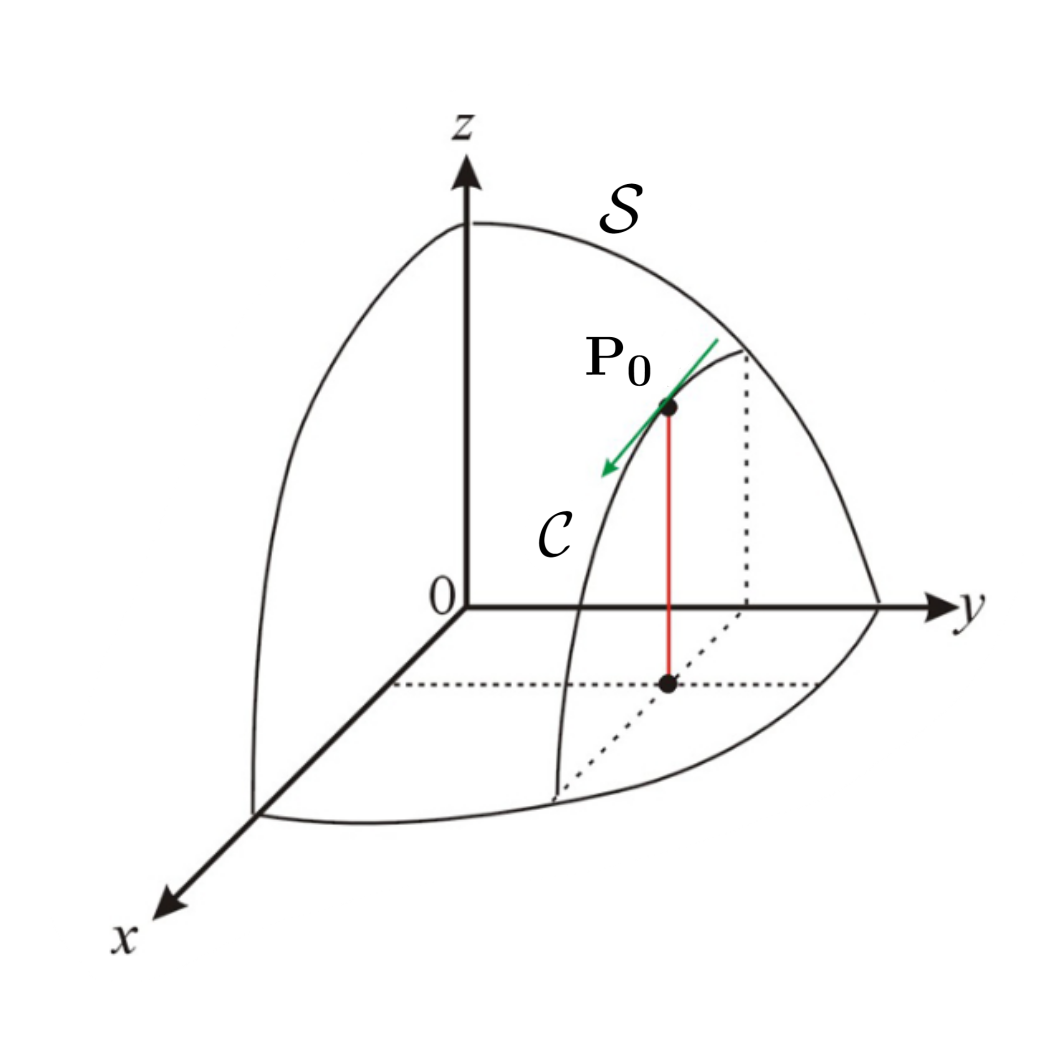
\includegraphics[width=0.45\textwidth]{figures/lec6.1.png}
  \caption{Geometric Meaning}
  \label{fig1:6}
\end{wrapfigure}

The partial derivative measures the change of a function at a point due to a particular variable, keeping all others constant. The geometry of partial derivatives is best visualized in 3 dimensions. Taking $f: \Op{2} \to \R$, we consider the surface $\mathcal{S} \subset \R^3$ defined by $z = f(x,y)$. Let $P_0 = (x_0, y_0, f(x_0, y_0))$ be a point on $\mathcal{S}$. Then the value $f_x(x_0, y_0)$ (if it exists) is the slope of the tangent to $\mathcal{S}$ at $(x_0, y_0, f(x_0, y_0))$ pointing in the positive x direction.

Another interpretation is to consider the plane

$\mathcal{P} = \{(x,y,z) \mid y = y_0\}$, and the curve $\mathcal{C}$ on surface $\mathcal{S}$ given by $\mathcal{C} = \mathcal{S} \cap \mathcal{P}$. Then, $f_x(x_0, y_0)$ is the slope of the tangent to the curve $\mathcal{C}$, in the direction of increasing x co-ordinate.

For $f: \Op{n} \to \R$ with $n > 2$, although it becomes harder to visualize, the interpretation remains the same.

\newpage

\section{Examples}

We now lay out some interesting and instructive examples, which would illustrate some general results about partial derivatives.

\begin{Eg}{}{}
  Consider $f: \R^2 \to \R$ given by $f(x,y) = x^3 + y^4 + \sin(xy)$. Then,
  $$\pdv{f}{x} = 3x^2 + y\cos{xy} \text{ and } \pdv{f}{y} = 4x^3 + x\cos{xy}$$
\end{Eg}

\begin{Eg}{}{}
  We know that Differentiable functions  $f: \Op{n} \to \R$ are continuous. However, even existence of all partial derivatives is too weak to ensure continuity.\\
  Consider $f: \R^2 \to \R$ given by
  $$f(x,y) = \frac{xy}{x^2 + y^2}$$
  Evidently, all the partial derivatives exist, but as shown previously, this function is discontinuous at $(0,0)$.
\end{Eg}

\begin{Def}{}{}
  A function $f: \Op{} \to \R$ is called $C^k(\mathcal{0})$ is all the \( {k}^{\text{th}} \) order partial derivatives exist and are continuous.
\end{Def}

\section{Higher Order Partial Derivatives}

Assume that partial derivatives of $f: \Op{n} \to \R$ exist in a neighbourhood of $a \in \Op{n} $. Then we can talk about the partial derivatives of $\pdv{f}{x_i}: \Op{n} \to \R$ at $a$. We denote:
\[f_{x_i x_j}(a) \equiv \pdv{f}{x_j} \mathrel{\mathop:}= \frac{\partial}{\partial x_j} \pdv{f}{x_i} = \lim_{h \to 0} \frac{1}{h} \left( \pdv{f}{x_i}\/(a+h e_i)- \pdv{f}{x_i}\/ (a) \right)
\]
We can define higher order partial derivatives similarly. Please note that the order of differentiation matters in general. For starters, of  $f_{x_i x_j}$ and $f_{x_j x_i}$, one may exist while the other may not. Also, even if both exist, they may not necessarily be equal over the entire domain. We leave it to the reader to find an example of the former case, and provide an example for the latter.

\begin{Eg}{}{}
  Consider $f: \R^2 \to \R$ given by
  \[
    f(x,y) =
    \begin{cases}
      \frac{xy(x^2 - y^2)}{x^2 + y^2} & (x,y) \neq (0,0) \\
      0                               & (x,y) = (0,0)
    \end{cases}
  \]
  In this case, it is easy to show (Exercise!) that both $f_{xy}$ and $f_{yx}$ exist, but
  \[f_{xy}(0,0) = 1 \neq -1 = f_{yx}(0,0)\]
\end{Eg}

\begin{Eg}{}{}
  However in many \emph{well-behaved} cases, we will find $f_{xy} = f_{yx}$.
  For instance, consider $f: \R^2 \to \R$ given by $f(x,y) = sin(x) + e^y + xy$. Show that $f_{xx} = f_{yy} = 1$ over $\R^2$.
\end{Eg}

Often, the dependence of the partial derivative on the order of differentiation is the exception rather than the rule. We now develop a sufficient condition for $f_{xy} = f_{yx}$ to hold.

\section{Clairaut's Theorem}

\begin{Thm}{Clairaut}{}\label{thm1:19}
  Let $(a,b) \in \Op{2}$ and $f:\Op{2} \to \R$. Suppose $f_x$, $f_y$, $f_{xy}$, and $f_{yx}$ all exist on $\Op{2}$. If $f_{xy}$ and $f_{yx}$ are continuous at $(a,b)$, then $f_{xy}(a,b) = f_{yx}(a,b)$.
\end{Thm}

\begin{proof}
  Without loss of generality, we take $(a,b) = (0,0) \in \Op{}^2$. As $\Op{}^2$ is open, we choose a box $[h,0]\times [0,k] \subset \Op{}^2$. Now, we have
  \begin{align*}
    f_{xy}(x,y)
     & = \pdv{f}{y}{x}\/(x,y) = \lim_{k \to 0} \frac{f_x(x,y+k) - f_x(x,y)}{k}                \\
     & = \lim_{k \to 0} \lim_{h \to 0} \frac{1}{hk}(f(x+h,y+k) - f(x,y+k) - f(x+h,y)+ f(x,y))
  \end{align*}
  We define
  \[F(h,k) = \frac{1}{hk}(f(h,k) - f(0,k) - f(h,0)+ f(0,0))\]
  Thus, by the above result, we have
  \begin{align*}
     & f_{xy}(x,y) = \lim_{k \to 0} \lim_{h \to 0} F(h,k) \text{, and similarly} \\ &f_{yx}(x,y) = \lim_{h \to 0} \lim_{k \to 0} F(h,k)
  \end{align*}
  Now we proceed for the proof in earnest. Define $f_1(x) = f(x,k) - f(x,0)$, which is continuous on $[0,h]$ and differentiable on $(0,h)$. Thus, by Lagrange's Mean Value Theorem, there exists $c_1 \in (0,h)$ (depending upon both $h$ and $k$), such that, $h(f_1'(c_1)) = (f_1(h) - f_1(0))$, i.e.
  \begin{align*}
    \therefore\; f_x(c_1,k) - f_x(c_1,0) & =  \frac{1}{h}(f(h,k) - f(0,k) - f(h,0)+ f(0,0)) = kF(h,k) \\
    \implies F(h,k)                      & = \frac{1}{k}(f_x(c_1,k) - f_x(c_1,0))
  \end{align*}
  Again, define $f_2(y) = f_x(c_1,y)$, which again satisfies all conditions for the Mean Value Theorem. Thus, there exists $c_2 \in (0,k)$ such that $k(f_2'(c_2)) = (f_2(k) - f_1(0))$, which gives, $F(h,k) = f_{xy}(c_1, c_2)$.\\
  Repeating this entire construction, we can find $(c_1', c_2') \in [0,h]\times[0,k]$ such that $F(h,k) = f_{yx}(c_1', c_2')$.\\
  Thus, $f_{xy}(c_1, c_2) = f_{yx}(c_1', c_2')$. But, $0 < c_1, c_1' < h$ and $0 < c_2, c_2' < k$. Thus, as $(h,k)$ can be made arbitrarily small, taking  $(h,k) \to 0$, we have
  \[
    \lim_{(c_1, c_2) to 0} f_{xy}(c_1, c_2) = \lim_{(c_1', c_2') to 0} f_{yx}(c_1', c_2')
  \]
  By the continuity of $f_{xy}$ and $f_{yx}$, we have $\mathbf{f_{xy}(0,0) = f_{yx}(0,0)}$.

\end{proof}

\msk

In particular, $f_{xy} = f_{yx}$ for $C^2$ functions over a given domain. In the next lecture, we sharpen this result slightly, and relate the  partial derivatives to the total derivative.


\end{document}
